\documentclass[12pt,a4paper]{article}
\usepackage[utf8]{inputenc}
\usepackage{amsmath}
\usepackage{amsfonts}
\usepackage{amssymb}
\usepackage{graphicx}
\usepackage[left=1cm,right=1cm,top=1cm,bottom=2cm]{geometry}
\usepackage{xcolor}
\usepackage{subcaption}
\usepackage{listings}
\usepackage{tabularx}
\usepackage{gensymb}
\usepackage{verbatim}
%\usepackage{subfig}
\usepackage{mathtools}
\usepackage{mathdefs}
\usepackage{placeins}
\usepackage{float}

\usepackage{amsthm}
\usepackage{graphicx}
%\usepackage{subfigure}
\usepackage{mathdefs}
\usepackage{algpseudocode}
\usepackage{algorithm}
\usepackage{bm}
\usepackage{bbm}
\usepackage{kbordermatrix}
\usepackage{mathdefs}
\usepackage{mathrsfs}
\usepackage{multirow}

\usepackage{hyperref}
\usepackage{cleveref}

\newtheorem{remark}{Remark}
\newtheorem{corollary}{Corollary}
\newtheorem{definition}{Definition}
\newtheorem{example}{Example}
\newtheorem{fact}{Fact}
\newtheorem{lemma}{Lemma}
\newtheorem{proposition}{Proposition}
\newtheorem{theorem}{Theorem}

\newcommand{\assref}[1]{Ass.~\ref{ass:#1}}
\newcommand{\clmref}[1]{Claim~\ref{clm:#1}}
\newcommand{\conref}[1]{Conj.~\ref{con:#1}}
\newcommand{\corref}[1]{Cor.~\ref{cor:#1}}
\newcommand{\defref}[1]{Def.~\ref{def:#1}}
\newcommand{\exaref}[1]{Ex.~\ref{exa:#1}}
\newcommand{\facref}[1]{Fact~\ref{fac:#1}}
\newcommand{\lemref}[1]{Lem.~\ref{lem:#1}}
\newcommand{\prpref}[1]{Prop.~\ref{prp:#1}}
\newcommand{\thmref}[1]{Thm.~\ref{thm:#1}}
\newcommand{\eqnref}[1]{(\ref{eq:#1})}
\newcommand{\secref}[1]{\S\ref{sec:#1}}
\newcommand{\appref}[1]{App.~\ref{app:#1}}
\newcommand{\figref}[1]{Fig.~\ref{fig:#1}}
\newcommand{\tabref}[1]{Table~\ref{tab:#1}}
\newcommand{\algoref}[1]{Alg.~\ref{alg:#1}}
\newcommand{\remref}[1]{Remark~\ref{rem:#1}}

\hypersetup{colorlinks=false}
\hypersetup{colorlinks,citecolor=black,filecolor=black,linkcolor=black,urlcolor=black}\label{sr_1}


\DeclarePairedDelimiter\ceil{\lceil}{\rceil}
\DeclarePairedDelimiter\floor{\lfloor}{\rfloor}

% disable indent
\setlength\parindent{0pt}

\title{Probability of Dice Sequences}
\author{Jonathan Stokes}

\begin{document}
\maketitle

\hrulefill\\

In rolling $6$ dice what is the probability of rolling $1,2,3,4$? Or more generally in rolling $n$ dice what is the probability for rolling a length $m$ sequence starting with $1$?
It is straight forward to estimate the probability of rolling these sequences using $100,000$ monte carlo simulations per dice count, see \cref{fig:monte_carlo_sim}.\\

\begin{figure}[h]
    \centering
    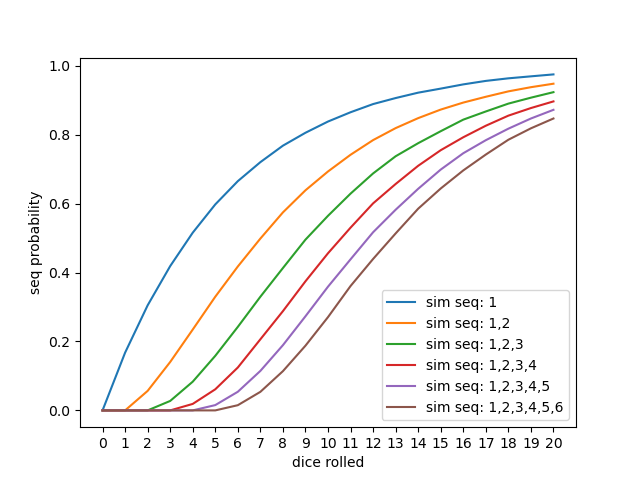
\includegraphics[width=0.5\textwidth]{figs/monte_carlo_seq_prob.png}
    \caption{}
    \label{fig:monte_carlo_sim}
\end{figure}

At first this looks similar the probability of drawing a straight in $5$ card draw poker. If one draws a straight in $5$ card draw poker including a royal flush there are 

\begin{enumerate}
\item $\binom{10}{1}$ ways to choose the low card in the straight, recalling that the ace may be $1$ or follow the king in a straight. 
\item $\binom{4}{1}^5$ ways to select the card suits.
\end{enumerate}
and generally there are $\binom{52}{5}$ ways of drawing $5$ cards. So the probability of drawing the straight in $5$ card draw poker is
\begin{equation}
\frac{\binom{10}{1}\binom{4}{1}^5}{\binom{52}{5}} \approx 0.00394
\end{equation}

So generalizing the probability of drawing a length $n$ straight for $n\in\{2 \ldots 13\}$ is 
\begin{equation}
\frac{\binom{15-n}{1}\binom{4}{1}^n}{\binom{52}{n}}
\end{equation}

Now lets try applying this same logic to the probability of rolling a length $m$ sequence in a roll of $n$ dice for $n\geq m$ dropping the requirement that the sequence start at $1$.
\begin{enumerate}
\item $\binom{7-m}{1}$ ways to choose the low number in the sequence.
\item $\binom{6}{1}^{n-m}$ ways to roll the remaining dice.
\end{enumerate}
and generally there are $\binom{6}{1}^n$ ways of rolling $n$ dice. Therefore the probability of rolling a length $m$ sequence in a roll of $n$ dice is,
\begin{equation}
\frac{\binom{7-m}{1}\binom{6}{1}^{n-m}}{\binom{6}{1}^n} = \frac{\binom{7-m}{1}}{\binom{6}{1}^m} = \frac{7-m}{6^m}
\label{eq:wrong_eq}
\end{equation}
which looking at \cref{fig:monte_carlo_sim} is clearly incorrect for $m=6$ and sequence $1,2,3,4,5,6$ as \cref{eq:wrong_eq} is constant in $n$ the number of dice rolled.\\

What did we do wrong? The term $\binom{7-m}{1}$ implicitly assumes that on any roll of the dice there are always $6$ different numbers to choose from. In the case of cards this type of assumption is correct 
since every deck of has $13$ distinct values ($14$ if the ace can be low and high). However in the case of a roll of $6$ dice we may not roll a $1$ leaving only $5$ numbers to choose from in which case there
are not $\binom{7-m}{1}$ ways to choose the lowest number in the sequence.\\

\hrulefill\\

So what is the solution? Well the short answer is that I have not worked out a closed for solution for the general case of a sequence of length $m$ starting at $1$. However below I give a solution
for the case where $m=2$.\\

What is the probability of rolling a $1$ and a $2$ when rolling $3$ dice? First lets define the following events.
\begin{equation}
A \text{: 1 does appear in a roll of 3 dice.}
\end{equation}
\begin{equation}
B \text{: 2 does appear in a roll of 3 dice.}
\end{equation}

To find the probability of events $A$ and $B$ we need to find the probability of $\neg A$ and $\neg B$ which is the probability of rolling any of the other $5$ dice faces of the $3$ independent dice. Therefore
\begin{equation}
P(\neg A) = P(\neg B) = \left(\frac{5}{6}\right)^3
\label{eq:prob_not_one}
\end{equation}

and by analogy the probability of not rolling a $1$ and a $2$ is
\begin{equation}
P(\neg A \cap \neg B) = \left(\frac{4}{6}\right)^3
\label{eq:prob_one_and_two}
\end{equation}

It follows from \cref{eq:prob_not_one} that the probability of rolling either a $1$ or a $2$ is
\begin{equation}
P(A) = P(B) = 1-P(A) = 1 - \left(\frac{5}{6}\right)^3 = \frac{91}{216}
\end{equation}
To answer our initial question above we need to find $P(A \cap B)$.\\

Given \cref{eq:prob_one_and_two} the conditional probability of not rolling a $1$ given not rolling a $2$ is
\begin{align}
P(\neg A| \neg B)   &= \frac{P(\neg A \cap \neg B)}{P(\neg B)} = \frac{\left(\frac{4}{6}\right)^3}{\left(\frac{5}{6}\right)^3} = \left(\frac{4}{5}\right)^3
\label{eq:not_one_given_not_two}
\end{align}
and given the law of total probability
\begin{equation}
P(A) = P(A|B)P(B)+P(A|\neg B)P(\neg B)
\end{equation}
Therefore from \cref{eq:not_one_given_not_two} and since $P(A|\neg B) + P(\neg A|\neg B) = 1$,
\begin{align}
P(A|B)  &= \frac{P(A) - P(A|\neg B)P(\neg B)}{P(B)}\\
        &= \frac{P(A) - (1 - P(\neg A|\neg B))P(\neg B)}{P(B)}\\
        &= \frac{\left(1-\left(\frac{5}{6}\right)^3\right) - \left(1-\left(\frac{4}{5}\right)^3\right)\left(\frac{5}{6}\right)^3}{1-\left(\frac{5}{6}\right)^3}
        = \frac{30}{91}
\label{eq:A_cond_B}
\end{align}
and it follows that
\begin{equation}
P(A \cap B) = P(A|B)P(B) = \left(\frac{30}{91}\right) \left(\frac{91}{216}\right) = \frac{5}{36} \approx 0.138
\label{eq:A_and_B}
\end{equation}
Looking at \cref{fig:monte_carlo_sim} this looks about right.\\

Also notice given \cref{eq:A_cond_B} and \cref{eq:A_and_B} it follows that
\begin{align}
P(A \cap B)     &= P(A|B)P(B)\\
                &= P(A) - P(A|\neg B) P(\neg B)\\
                &= P(A) - (1 - P(\neg A|\neg B)) P(\neg B)\\
                &= P(A) - P(\neg B) + P(\neg A \cap \neg B)
\label{eq:reduced_A_and_B}
\end{align}

Now given \cref{eq:reduced_A_and_B} does this generalize for $n\geq 2$ dice rolled? Lets first define the following events
\begin{equation}
A_n \text{: 1 does appear in a roll of $n$ dice.}
\end{equation}
\begin{equation}
B_n \text{: 2 does appear in a roll of $n$ dice.}
\end{equation}

\begin{align*}
P(A_n \cap B_n) &= P(A_n) - P(\neg B_n) + P(\neg A_n \cap \neg B_n)\\
                &=  1-\left(\frac{5}{6}\right)^n -\left(\frac{5}{6}\right)^n + \left(\frac{4}{6}\right)^n\\
                &= 1 - 2\left(\frac{5}{6}\right)^n + \left(\frac{2}{3}\right)^n
\label{eq:A_and_B_sol}
\end{align*}
and as $n\to\infty$, $P(A_n \cap B_n) \to 1$ as expected.\\

\begin{figure}[h]
    \centering
    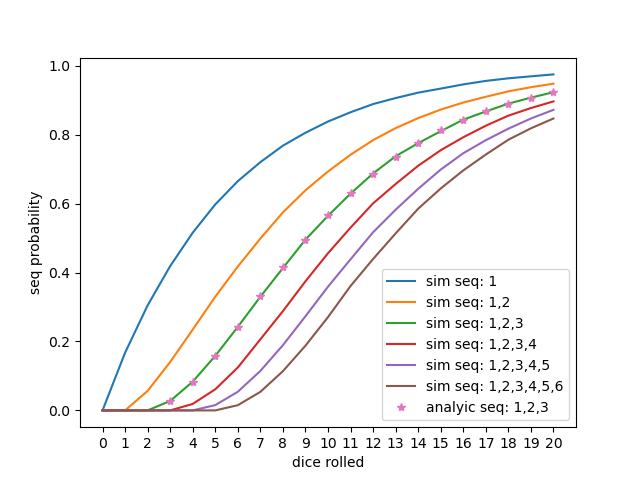
\includegraphics[width=0.5\textwidth]{figs/compare_analytic_sim.png}
    \caption{}
    \label{fig:compare_analytic_sim}
\end{figure}
\Cref{fig:compare_analytic_sim} compares the analytic and simulated results and as expected the simulated and analytical results are very close.\\

\hrulefill\\

Can this be generalized to the case of a length $m$ sequence? Lets first consider the case where $m=3$ In this case, replacing $B$ with $B \cap C$ \cref{eq:reduced_A_and_B} gives,\\

\begin{align}
P(A_n \cap B_n \cap C_n)    &= P(A_n) - P(\neg B_n) - P(\neg C_n)\\
                            &+ P(\neg A_n \cap \neg B_n) + P(\neg A_n \cap \neg C_n) + P(\neg B_n \cap \neg C_n)\\ 
                            &- P(\neg A_n \cap \neg B_n \cap \neg C_n)\\
                            &= 1 - 3\left(\frac{5}{6}\right)^n + 3\left(\frac{4}{6}\right)^n - \left(\frac{3}{6}\right)^n
\label{eq:A_and_B_and_C_sol}
\end{align}
Now given \cref{eq:A_and_B_sol} and \cref{eq:A_and_B_and_C_sol} by induction we can derive a closed form solution. Now say we want to know the probability of rolling the sequence of dice $1$ to $m$ where $m\in\{1,2,3,4,5,6\}$. Given $n\geq m$ lets define the events
\begin{equation}
A_{n,i} \text{: $i$ appears in a roll of $n$ dice.}
\end{equation}
for $i \in \{1\ldots m\}$.\\

So the probability of a sequence of length $m$ starting at $1$ appearing in a given roll of the dice is,
\begin{equation}
P\left(\bigcap_{i=0}^m A_{n,i}\right) = (-1)^i \binom{m}{i}\left( \frac{6-i}{6} \right)^n
\end{equation}

Using this equation to compute the analytic probability of rolling a dice sequence starting at $1$ of length $m$ and comparing these to the simulated results gives.

\begin{figure}[h]
    \centering
    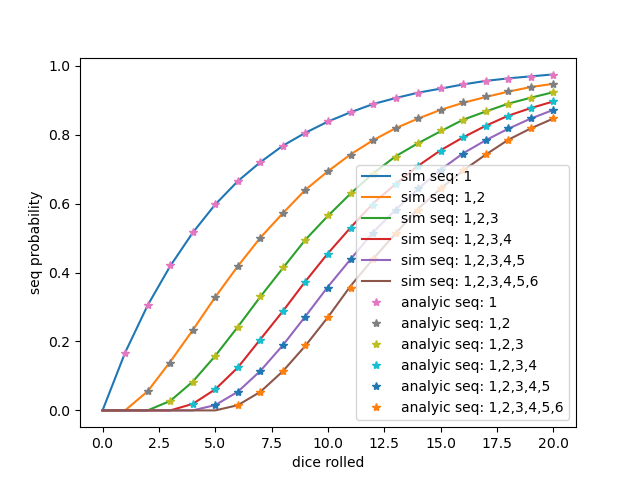
\includegraphics[width=0.5\textwidth]{figs/full_compare_analytic_sim.png}
    \caption{}
    \label{fig:full_compare_analytic_sim}
\end{figure}

\end{document}
